\chapter{Dokumentation for seriel kommunikation}

\section{Indleding}
I wineprep projektet skal der bruges en linux platform, som i dette projekt består af et DevKit8000 (DK8k) hvorpå der er installeret distributionen Ångstöm. 
Denne skal tage imod input fra brugeren af systemet via en grafisk brugergrænseflade og omskrive disse til kommandoer, som sendes til PSoC. Desuden
vil PSoC sende status beskeder tilbage til DK8k.
Der vil i projektet indgå en PSoC, som står for kommunikationen med DK8k samt for nogle af systemets motorer og sensorer,
men på grund af et begrænset antal GPIO-pinde og UDB'er på PSoC, vil det blive nødvendigt med to ekstra PSoCs, som kan tage sig af kommunikationen med de 
øvrige motorer og sensorer i systemet. Der vil derfor blive lavet en forbindelse mellem de tre PSoC-enheder, hvor PSoC'en, som tager imod kommandoer fra
DK8k, vil fungere som master over de to øvrige PSoCs. Der vil i denne dokumentation blive refereret til disse PSoC-enheder som MASTER
(forbindes til Devkit), TOP (slave til MASTER, som i sidder i toppen af Wineprep) og BOTTOM (slave til MASTER, som sidder i bunden af
Wineprep).
Ovenstående taget i betragtning vil det blive nødvendigt at etablere en tovejsforbindelse imellem DK8k og MASTER, samt en tovejsforbindelse imellem 
MASTER og TOP, samt MASTER og BOTTOM. 

Dette kan gøres på flere forskellige måder, f.eks. med en UART-protokol som på tidligere semester projekter. Der er i fagene HAL og GFV på 3. semester 
blevet arbejdet en del med de to serielle dataforbindelsesstandarder I2C og SPI, og det vil derfor være nærliggende at benytte en af disse to. 
Det er fra gruppens side og med opfordring fra vejleder blevet besluttet, at SPI vil blive benyttet i dette projekt til forbindelsen imellem DK8k og 
PSoC. Grunden til dette valg er mest af alt bekvemmelighed, da der allerede er arbejdet med SPI drivere til Linux og PSoC i tidligere laboratorieøvelser.   

\section{Design og implementering}
SPI er en synkron dataopførselsmetode, hvor to enheder indgår i et master/slave-forhold, og hvor data sendes og modtages mellem de to enheder på
samme tid med klokken som "taktstok". For mere information omkring SPI-protokollen henvises til bilag(*referance til SPI-protokollen).
DK8k vil i dette tilfælde udføre rollen som master i forbindelsen til MASTER, hvilket også betyder, at det er denne, som står for at starte 
dataoverførslen mellem de to enheder. Ligeledes vil MASTER fungere som master i forbindelsen til TOP og BOTTOM.

\begin{figure}[H]
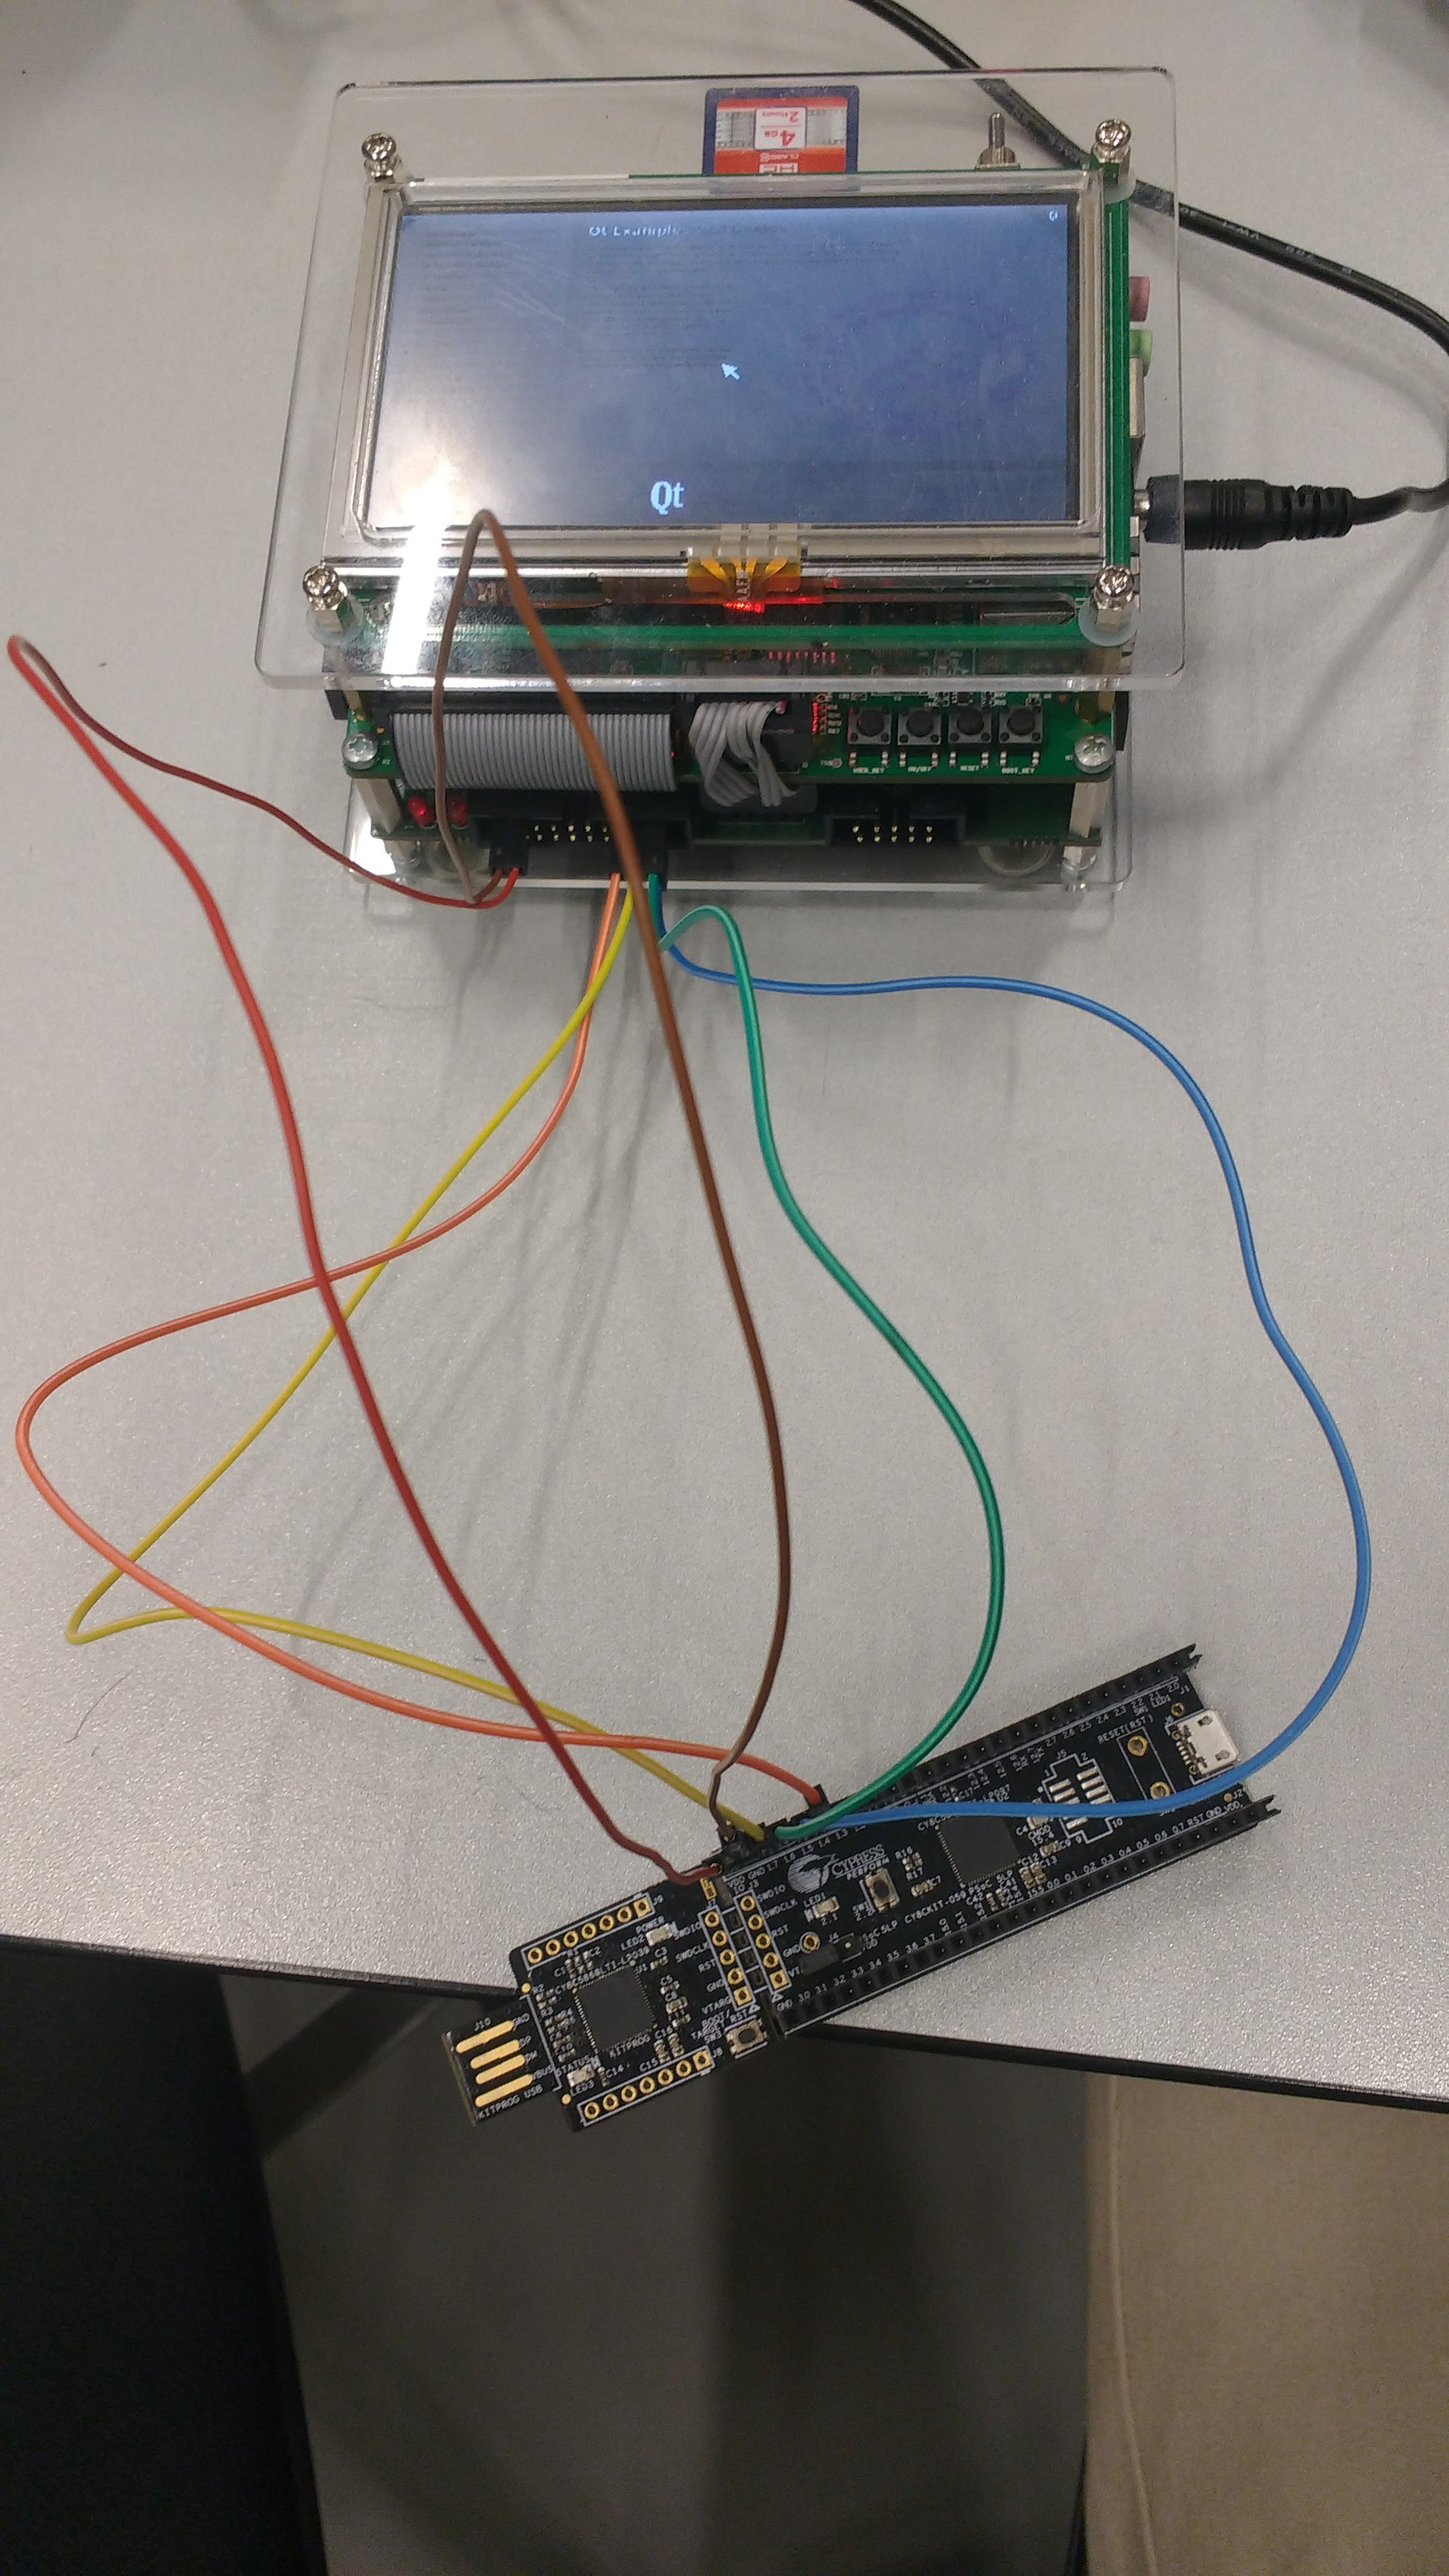
\includegraphics[scale=0.15]{Screenshots/Realisering_devkit_psoc}
\caption{Realisering af Devkit8000-PSoC SPI forbindelse}
\end{figure}

SPI undersøttes naturligvis af DK8k, men for at kunne etablere forbindelsen til MASTER skal den nødvendige SPI-driver skrives til Linux. 
Denne driver indeholder blandt andet den korrekte opsætning for forbindelsen samt implementeringen af SPI-metoderne til at sende/modtage data.
Der skal også skrives en character device driver, der gør det muligt for et program i userspace at tilgå SPI driveren. Der laves også en hotplug-driver,
der gør det muligt at indsætte PSoC i runtime. For mere information omkring implementeringen af denne driver samt eksempel på dens anvendelse henvises der til HAL 
øvelse 6 i bilag.
Vi har i dette projekt anvendt den SPI-driver, som er blevet udleveret på redmine i faget HAL. Så SPI-driver-modulerne indsættes blot på DK8k, og der 
laves de nødvendige device-noder. Disse noder er nødvendige for at kunne kommunikere mellem user- og kernelspace. 

\begin{figure}[H]
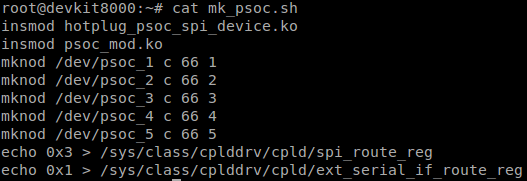
\includegraphics[scale=0.9]{Screenshots/Devkit_cat_mk_psoc}
\caption{Indsættelse af moduler i Linux kernen og oprettelse af device noder}
\end{figure}

De tre PSoC-enheder skal ligesom DK8k også have implementeret software, der kan håndtere SPI-forbindelsen og reagere
på den ønskede måde, når der modtages data. Denne software skrives med værktøjet PSoC Creator, som via et simpelt drag-and-drop interface gør det
nemt at konfigurere SPI. Selve SPI-driveren skal derfor ikke skrives, men der skal laves en source-fil, hvori det er muligt at kalde metoder til
styring af SPI, håndtere Rx-interrupts og anvende de modtagne data til at udføre forskellige opgaver for systemet.

\begin{figure}[H]
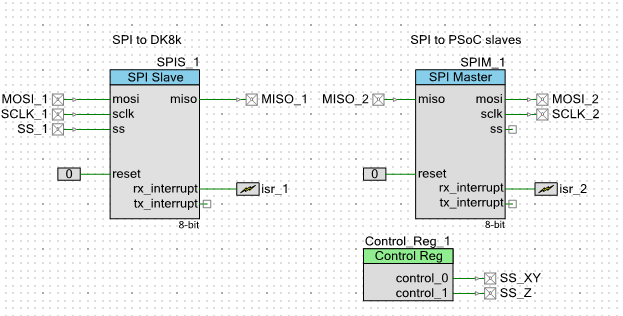
\includegraphics[scale=0.8]{Screenshots/PSOC_opstilling_spi}
\caption{Topdesign for PSoC1}
\end{figure}

MASTER skal have både et SPI-master- (SPIM) og et SPI-slave-modul (SPIS) i PSoC Creator. Der ønskes et interrupt ved Rx på SPIS, da slaven skal reagere
hver gang der modtages data fra master, hvorefter der skal skrives tilbage og udføres en opgave. Dette vil blive håndteret i en interruptrutine af en switch 
implementation, der kaldes hver gang Rx-interruptflaget går højt. SPI-driveren på DK8k er opsat således, at der sendes 16 bits til MASTER.
Af disse er de første 8 bit tiltænkt adresse- og kommandobits, og de næste 8 bit er selve data. Der vil i main først blive switched på adresse-bits,
som fortæller hvilket device, der benyttes. Da der kun er én PSoC som slave til DK8k, vil et forsøg på at skrive til et andet device, end det, der er blevet
afsat til MASTER, returnere en fejlmeddelelse. Kommandobits indikerer, om der ønskes status læst tilbage fra MASTER, eller om det blot er 
tilstækkeligt, at MASTER behandler den modtagne kommando og sender nogle default-værdier tilbage. Mere specifikt vil MASTER fungere som formidler af
kommandoer mellem DK8k og TOP og BOTTOM. MASTER vil ikke indeholde nogen anden særegen funktionalitet, da den ikke har direkte adgang til motorer, sensorer, osv.
Disse eksterne komponenter håndteres af TOP og BOTTOM på baggrund af de kommandoer, der sendes fra DK8k til MASTER. Inde i den føromtalte switch vil MASTER
behandle disse kommandoer ved at påføre TOP eller BOTTOM en pågældende opgave vha. metoder fra SPIM. SPIM's Rx-interruptflag går ligeledes højt, når
TOP/BOTTOM rapporterer deres status tilbage. Da vil der i en interruptrutine også være switch, som behandler disse status-meddelelse. MASTER's rolle kunne passende
beskrives ved et tilstandsdiagram (*referer til applikationsmodel, når denne engang er opdateret).

\begin{figure}[H]
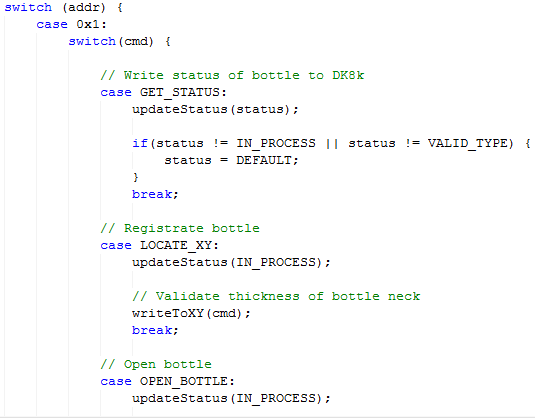
\includegraphics[scale=0.9]{Screenshots/PSOC_switch}
\caption{Eksempel på en switch statement i PSoC koden}
\end{figure}

Topdesign og koden for TOP og BOTTOM vil blive implementeret næsten på samme måde som MASTER mht. kommunikationen med denne, hvor der implementeres et Rx-interrupt
og en switch som behandler den modtagne data. De to slave-PSoC-enheder vil dog kun have et SPIS modul implementeret, og derfor have færre switch-cases.
Der bruges en 8bit kommando til at sende data til TOP og BOTTOM, og det er denne kommando, som bliver switched på. Når en opgave er udført, eller der er opstået
en fejl, opdateres Tx-bufferen med en relevant status-meddelelse. Dette sker løbende i udørelsen af en pågældende opgave.
\begin{figure}[H]
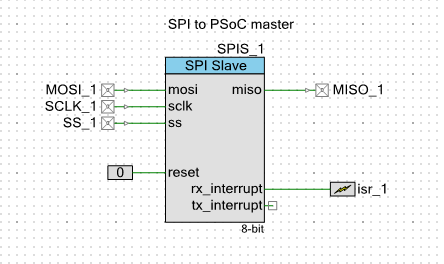
\includegraphics{Screenshots/PSOC_topdesign_SPIS}
\caption{Topdesing for PSoC2 og PSoC3}
\end{figure}

\begin{figure}[H]
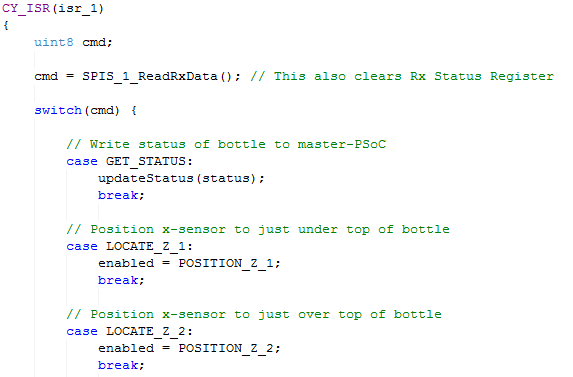
\includegraphics[scale=0.9]{Screenshots/PSOC_switch_slave}
\caption{Eksempel på switch cases for PSoC2 og PSoC3}
\end{figure}     
 
\section{Test}

\subsection{Test af SPI forbindelse mellem MASTER og PSoC-slave}

Testen for forbindelsen mellem MASTER og PSoC-slave gennemføres vha. en terminal og logic analizer på Analog Discovery. De to PSoC-enheder bliver sat 
til hver deres PC, og der laves en UART-forbindelse, så det kan ses på et terminalvindue, hvilke data, der bliver sendt og modtaget. Derefter forbindes de to PSoC-
enheder til hinanden med SPI, og der tilføjes desuden en fælles stelforbindelse. Hvor MASTER normalvist modtager sine kommandoer fra DK8k, vil den i denne test
modtage disse fra brugeren via terminalvinduet på den ene PC. PSoC-slave er blot en test-dummy, som modtager denne kommando og udskriver den på terminalvinduet
på den anden PC, og skriver den i Tx-bufferen, så MASTER kan læse den igen og udskrive den på sit terminalvindue. Derved testes tovejskommunikationen mellem PSoC'ene.
På billedet ses også en VDD-forbindelse fra MASTER, denne er dog kun nødvendig, hvis slaven ikke får VDD fra PC.
 
\begin{figure}[H]
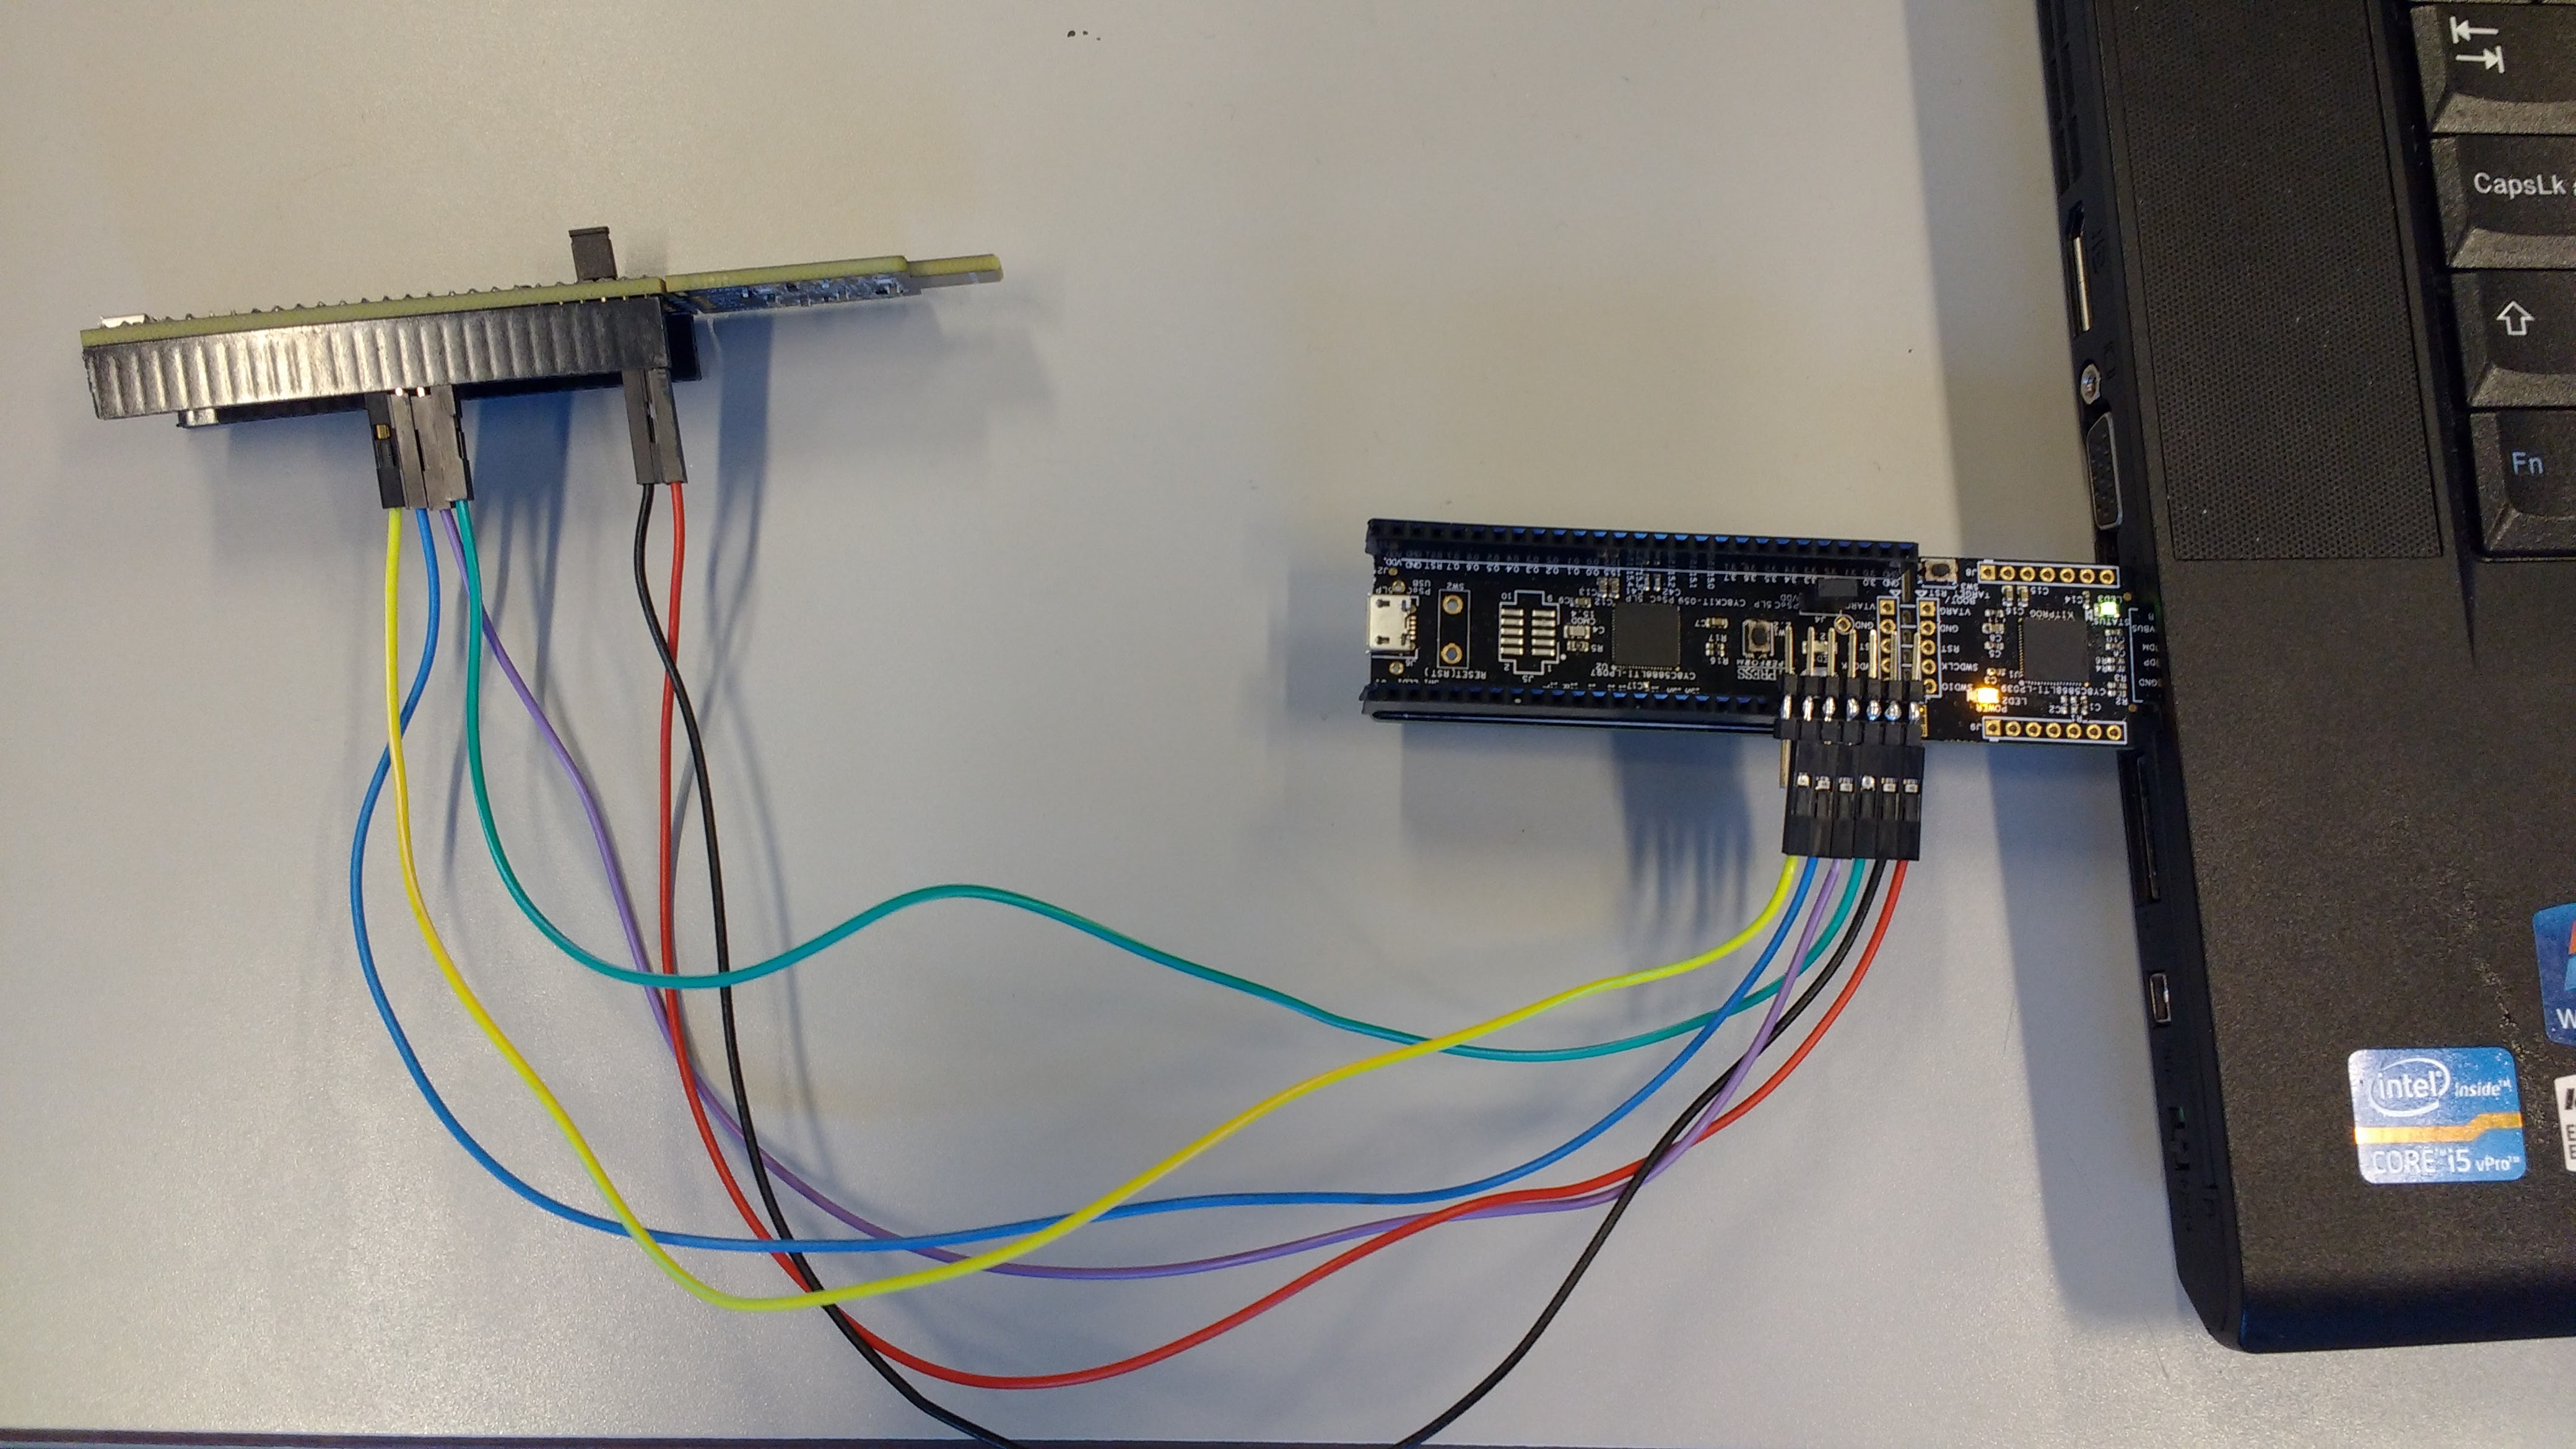
\includegraphics[scale=0.9]{Screenshots/SPI_testopstilling}
\caption{PSoC forbundet til PC via UART og med anden PSoC-enhed via SPI}
\end{figure}

Desuden sættes Analog Discovery på SPI-forbindelsen, og der måles på CLCK, SS (slave select) og MOSI for at sikre, at SPI-signalet ser fornuftigt ud. Altså at SS 
går lav ved dataoverførsel, og den korrekte bitsekvens sendes på MOSI. Grunden til, at der ses efter, om SS går lav, er fordi, der ved SPI kan være flere slaver 
tilsluttet. SPI fungerer på den måde, at den trækker signalet lavt på den slave, som skal modtage signalet.
CLCK er ikke særligt interessant, men det kan evt. tjekkes om frekvensen stemmer overens med det, som angives i koden for PSoC.

\begin{figure}[H]
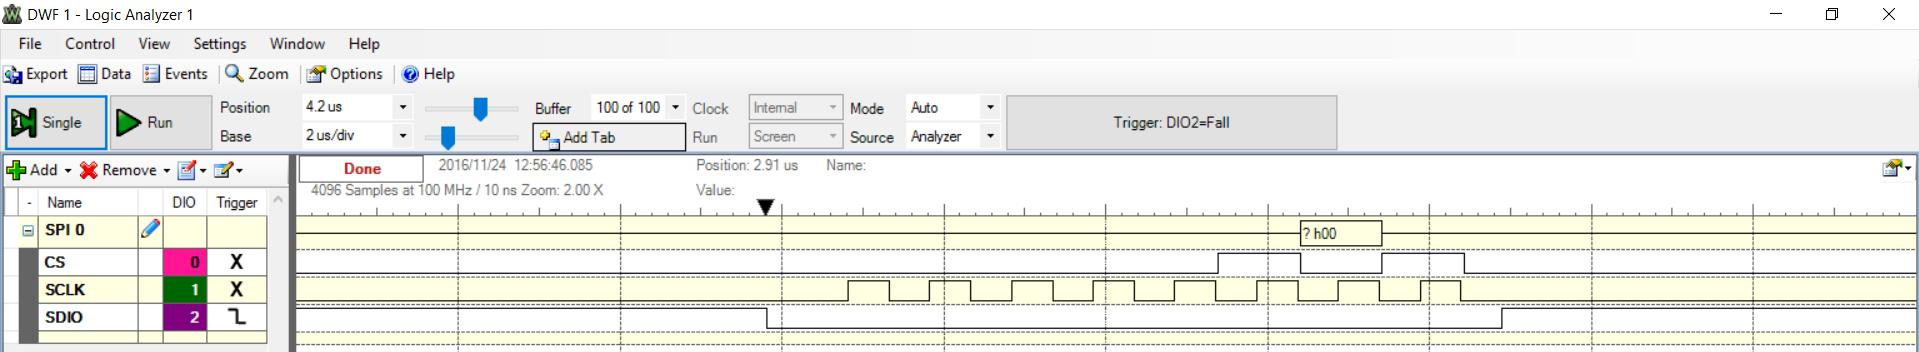
\includegraphics[scale=0.9]{Screenshots/Logic_analyzer}
\caption{Test med Analog Discovery på SPI-forbindelsen}
\end{figure}

Der sendes data fra MASTER til slave, og der kigges på terminalen og logic analizer for at se hvilke data, slave modtager. I denne test sendes kommandoen 0x05 til 
slaven at antal gange.

\subsection{Test af SPI-forbindelse imellem DK8k og MASTER}

Testen for SPI-forbindelsen imellem DK8k og MASTER foretages med Analog Discovery, hvor der måles på SS, CLCK, og henholdsvis MISO og MOSI.

\begin{figure}[H]
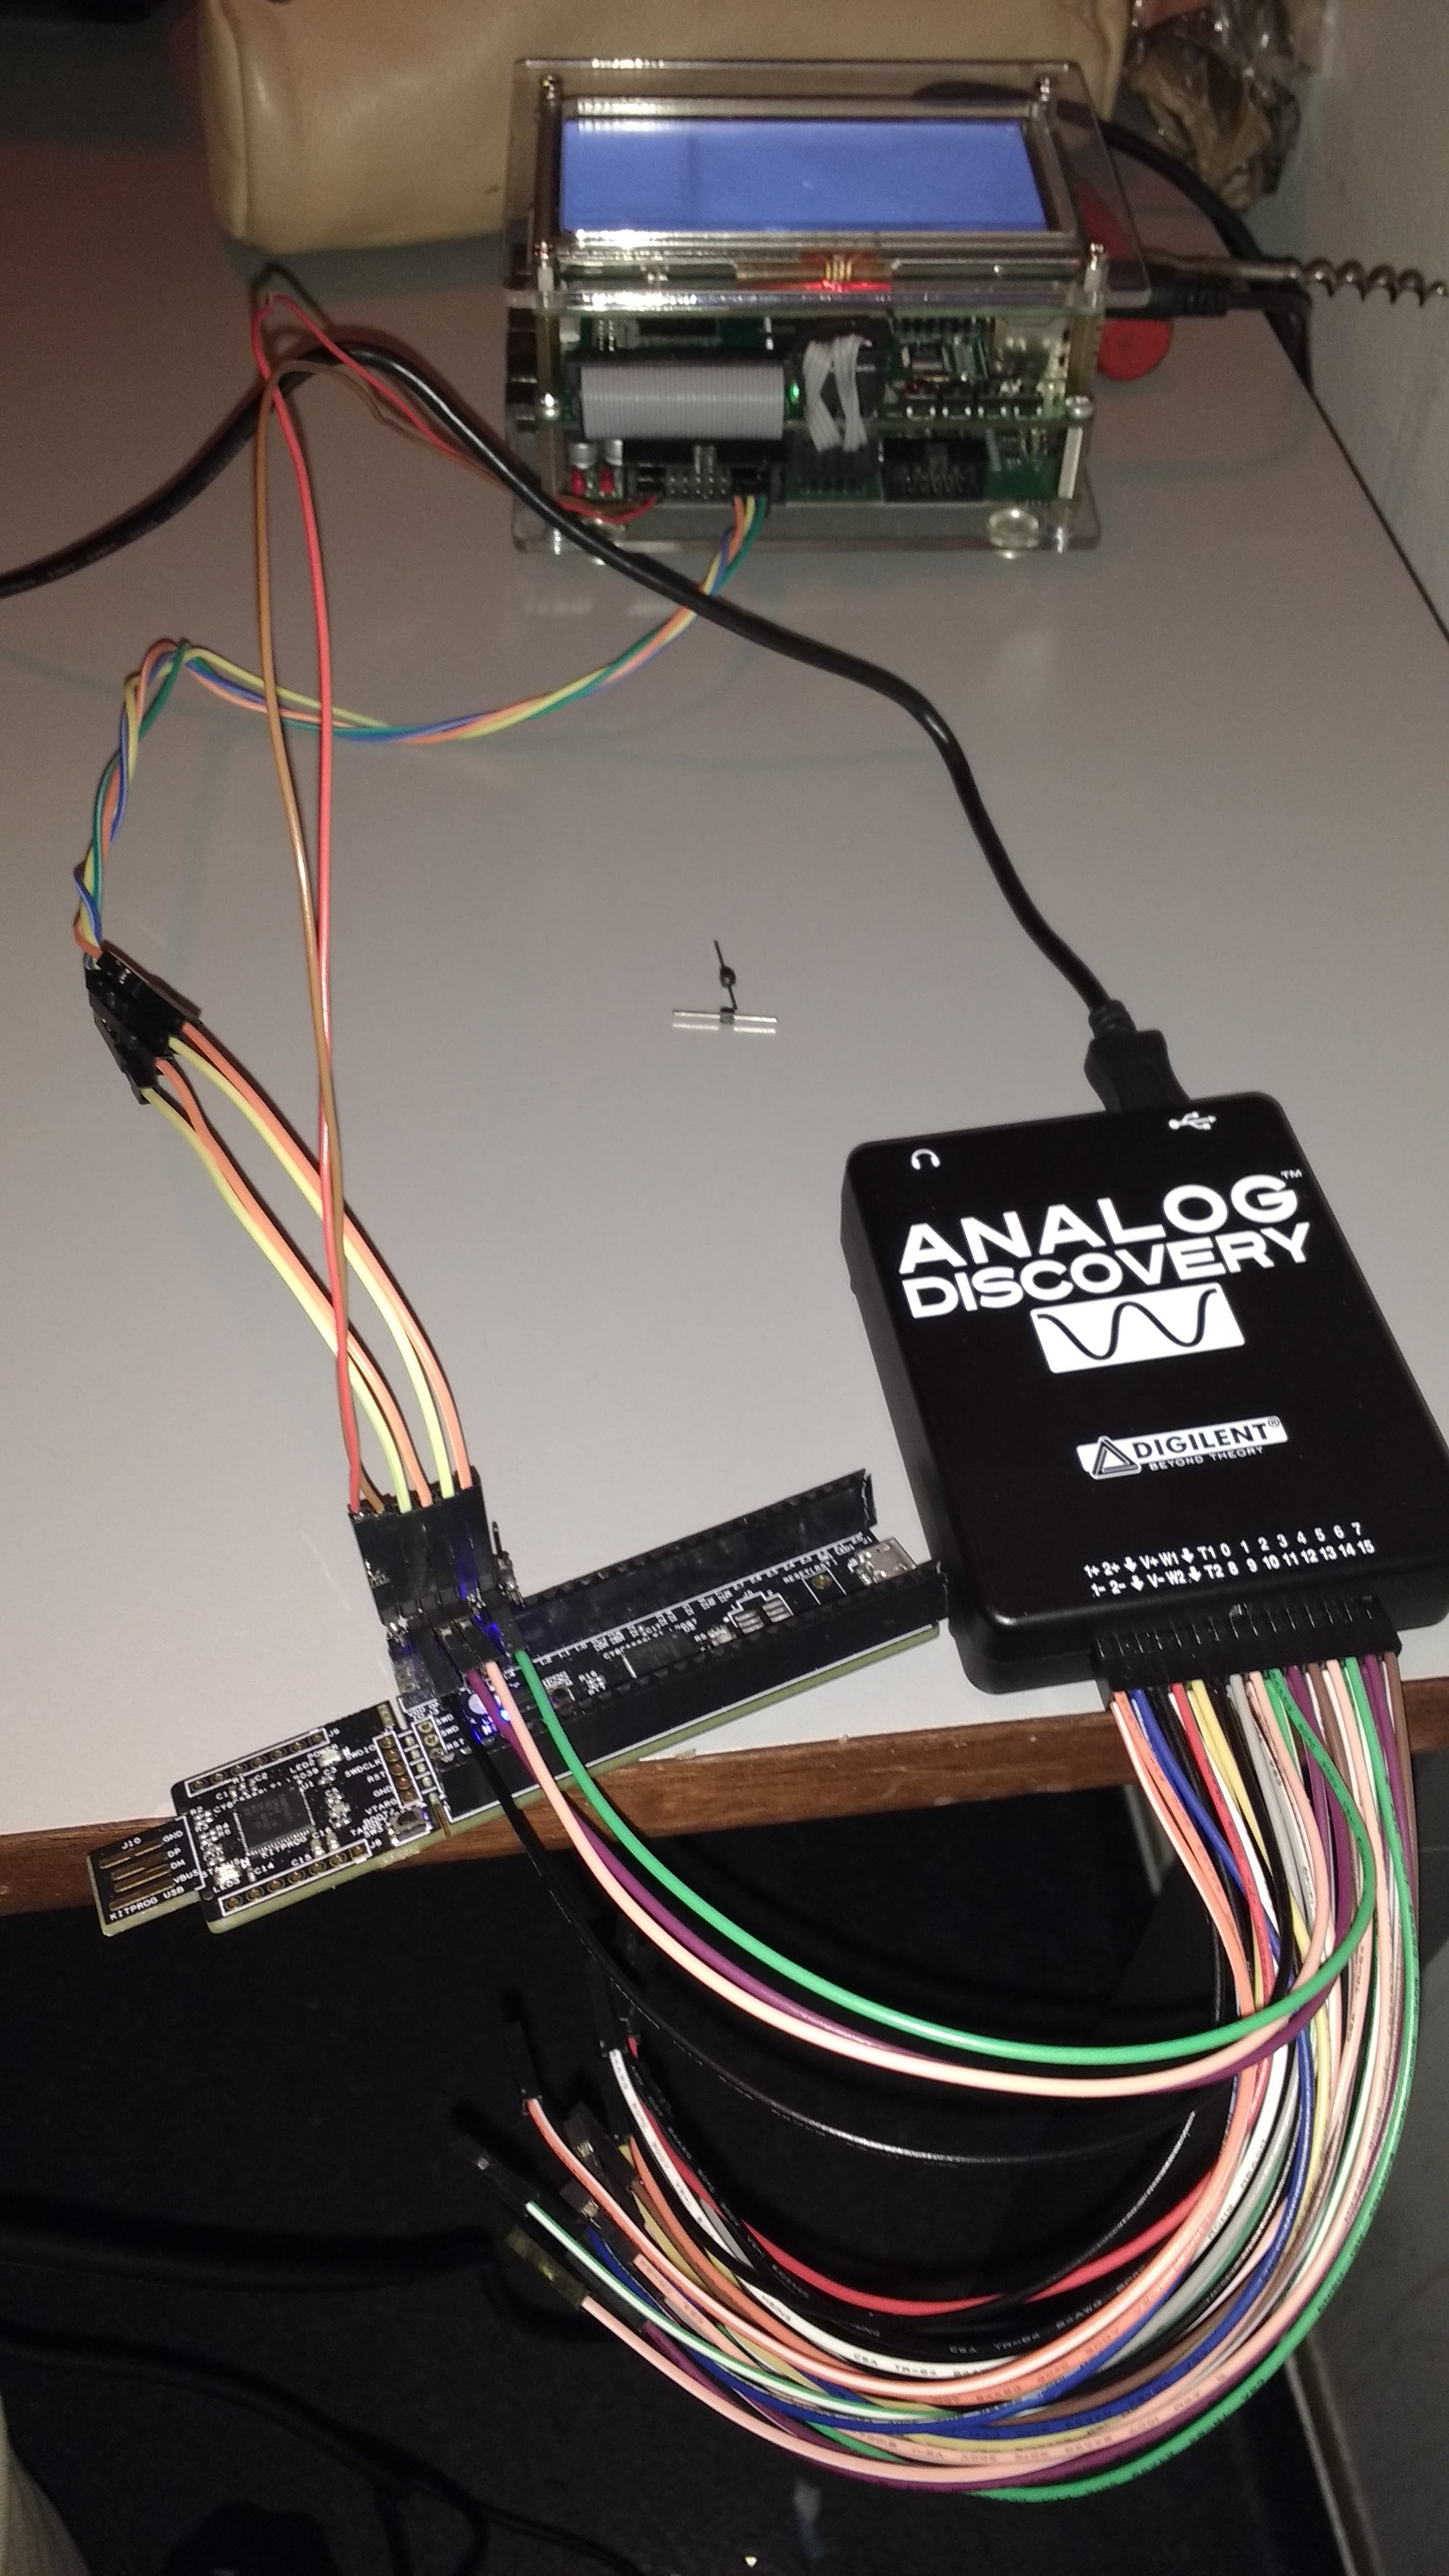
\includegraphics[scale=0.9]{Screenshots/Test_analog}
\caption{Opstilling med Analog Discovery til test af SPI-forbindelse} 
\end{figure}

Der udføres to test-scenarier. I første test sendes data fra DK8k (master) og der foretages en måling på MOSI forbindelsen med logic analyzer-
funktionen på Analog Discovery. Denne test skal sikre, at vi får sendt de korrekte adresse- og data-bits over til MASTER, samt at SS og CLCK opfører sig 
som ønsket. Det vil sige at SS går lav ved dataoverførsel og at CLCK er stabil. I denne test bruges Linux-terminalen på DK8k til at sende nogle forskellige
værdier til MASTER med Linux-kommandoen echo, hvorefter der aflæses bit-kombinationer på logic analyzer.

I den anden test læses der fortsat på MOSI forbindelsen, og Linux-kommandoen cat bruges til at læse fra MASTER. Her aflæses det på terminalen, hvad der bliver sendt 
fra MASTER. I test-programmet på MASTER er der implementeret en switch, som gør, at når der læses med kommandoen cat PSoC{\_}5 fra Linux-terminalen, vil 
status på knap 2.1 på MASTER blive aflæst. Således kan det testes, at der sendes den korrekte data fra MISO.


\section{Resultater}
\subsection(Resultater af test for PSoC-PSoC SPI)

Ved testen ses, at der udskrives 05 på terminalvindue for PSoC-slave. Dette passer fint med den kommando, der sendes fra MASTER. SPI-forbindelsen fungerer altså
fint.
 
\begin{figure}[H]
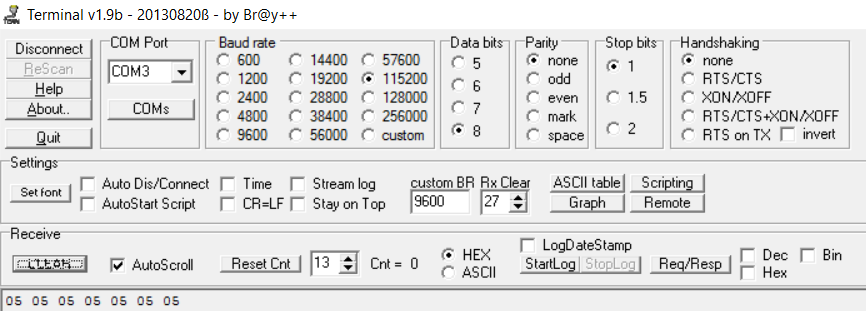
\includegraphics[scale=0.9]{Screenshots/Terminal_spi_slave}
\caption{Terminal udskrift fra PSoC-slave-enheden} 
\end{figure}  

Der kigges også på logic analizer, og det ses, at SS går lav ved dataoverførelse. Og der sendes desuden værdien 0x05 på MOSI. Igen virker det som forventet.
Det eneste problem ved denne test er, at MASTER først kan læse den sendte kommando efter at have sendt denne en tre-fem gange. Dette kunne give anledning til
problemer i den endelige implementering, da MASTER skal have klar besked om PSoC'enes status, da disses opgaver skal synkroniseres. En evt. "løsning" på dette
problem kunne være at indføre en "guard", f.eks en counter, som tjekker, at en kommando/meddelelse er blevet sendt/læst et vist antal gange, før der udføres
yderligere opgaver.

\begin{figure}[H]
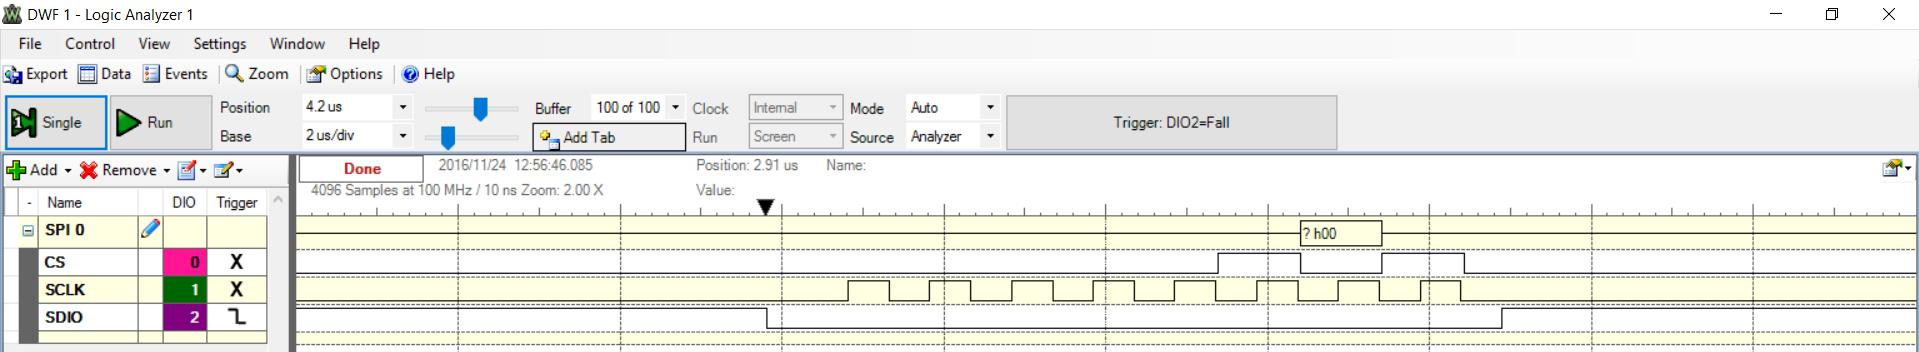
\includegraphics[scale=0.9]{Screenshots/Logic_analyzer}
\caption{logic analizer målt på SPI-forbindelsen} 
\end{figure} 

\subsection{Resultater af test for Devkit-PSoC SPI}
Ved første test-scenarie ses, hvordan der sendes værdien 20 fra DK8k til MASTER med Linux-kommandoen echo. På logic analyzer ses, at der sendes to gange 8 bit:
først en adresse kode, som er 65, og derefter værdien 20. Det ses også at SS går lav ved dataoverførsel, og at clock er stabil. Testen er derfor tilfredsstillende.
 
\begin{figure}[H]
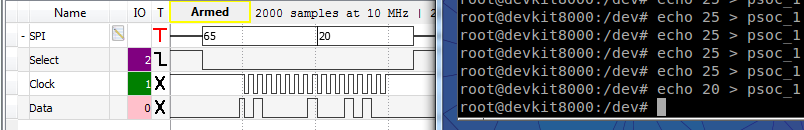
\includegraphics[scale=0.9]{Screenshots/Analog_devkit_echo_psoc_1}
\caption{Data bliver sendt fra DK8k til MASTER} 
\end{figure}

Ved det andet test-scenarie bruges Linux-kommandoen cat til at læse fra MASTER. Her ses, at der sendes en adresse-bit 5 og 0 via MOSI, og på terminalen ses
status for knappen på MASTER, som er trykket nede og derfor viser 1. 

\begin{figure}[H]
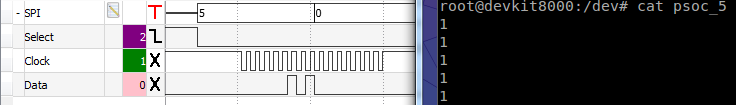
\includegraphics[scale=0.9]{Screenshots/Analog_cat_psoc_5}
\caption{Data bliver læst fra MASTER} 
\end{figure}

\section{Diskussion}
Ud fra ovenstående ses det at SPI kan bruges til at kommunikere imellem DK8k og MASTER, samt at kommunikere imellem PSoC-enhederne. Som resultaterne af 
testen viser, er SPI en smart måde, hvorpå der kan sendes og modtages data samtidigt. Det skal dog nævnes, at der har været mange problemer med denne kommunikation,
især ifb. med at læse data fra slave til master, og der er brugt adskillige timer på at få det til at virke. Så sammenlignet med UART, som fungerede problemfrit
på 1. og 2. semester, så har SPI været meget mere udfordrende at få til at virke.